%===================================== CHAP 4 =================================

\chapter{Experiment planning and results}
\label{chap:analysis}

\section{Experiment plans}
\label{sec:experiment_plan}

In this section we list the set of experiments we have performed in order to answer the research questions as stated in Section \ref{sec:problem_statement}. 


\subsection{Establishing Logistic Regression Baselines}

\begin{table}[h]
	\centering
	\caption{Our baseline experiments}
	\label{tab:experiments_baselines}
	\begin{tabular}{|l|l|l|l|}
		\textbf{Experiment Name}    & \textbf{Peers} & \textbf{Data per peer} & $\boldsymbol{\lambda}$      \\
		\hline
		Spam, centralized  & 1     & 3680 & $[2^{-8},2^{8}]$ \\
		Adult, centralized & 1     & 3000 & $[2^{-8},2^{8}]$ \\
		Susy, centralized  & 1     & 3000 & $[2^{-8},2^{8}]$
	\end{tabular}
\end{table}

These experiments were intended establish the best achievable performance with our implementation of logistic regression trained by SGD. They correspond to the traditional non-private and centralized training of classification models. Note that the results of these experiments may not be state-of-the-art for each data set, since we have not performed advanced feature extraction and selection. This is acceptable, since the intention of these experiments was to established a baseline that we can compare the models that are formed by our approach in a private and decentralized manner.


\subsection{Confirming Expected Effects of Differential Privacy}

In this project we have implemented training of a logistic regression, the aggregation mechanism guaranteeing differential privacy and the communication scheme that forms groups of peers to create aggregate models. When tuning the parameters of the implementation, we expected certain changes in the measured performance based on the theoretical and experimental results of previous work. The experiments in this section is intended to be validation of our implementation. In particular, we expected certain impacts when changing the privacy parameter $\epsilon$ and the regularization parameter $\lambda$. By confirming the expected behavior, we can have increased confidence in the correctness of our implementation, while also visualizing the dynamics of differential privacy.

\subsubsection{Changes in $\epsilon$}

The variance of the noise added when producing aggregated models is proportional to the parameter $\epsilon$. To confirm this behavior, we ran experiments with all parameters fixed except for $\epsilon$, which we tested over a wide range. Since noise is only added when locally trained models are aggregated, it was necessary to test with more than one participating peer.

\begin{table}[h]
	\centering
	\caption{Effects of privacy level}
	\label{tab:experiments_privacy_level}
	\begin{tabular}{|l|l|l|l|l|}
		\textbf{Experiment Name}            & \textbf{Peers} & \textbf{Data per peer} &
		 $\boldsymbol{\lambda}$ & $\boldsymbol{\epsilon}$                                              \\
		 \hline
		Spam, observing $\epsilon$ & 10    & 368  & $2^{-2}$  & $[2^{-8}, 2^{8}]$
	\end{tabular}
\end{table}

All the peers in this experiment collaborate to produce one aggregated model, and the full privacy budget is expended in the single aggregation. When the peers are tasked to label the test data, they use their local model and the aggregated model in an ensemble.

\subsubsection{Changes in $\lambda$}

As stated by Equation \ref{eq:aggregated_logistic_sensitivity}, the regularization parameter $\lambda$ is inversely proportional to the variance of the noise added to aggregated models. For this reason we expected that higher values of regularization should be help counter the detrimental effect of lower values of $\epsilon$. However, as regularization grows too large, predictive performance should degrade as the models become unable to fit to data. To confirm these effects, we tested wide ranges of regularization strength with different levels of privacy.

\begin{table}[h]
	\centering
	\caption{Effect of regularization strength}
	\label{tab:experiments_regularization_strength}
	\begin{tabular}{|l|l|l|l|l|}
		\textbf{Experiment Name}    & \textbf{Peers} & \textbf{Data per peer} & $\boldsymbol{\lambda}$         & $\boldsymbol{\epsilon}$ \\
		\hline
		Spam, observing $\lambda$, no privacy       & 10    & 368  & $[2^{-8}, 2^{3}]$ & $2^{10}$   \\
		Spam, observing $\lambda$, common privacy   & 10    & 368  & $[2^{-8}, 2^{3}]$ & $0.1$      \\
		Spam, observing $\lambda$, stronger privacy & 10    & 368  & $[2^{-8}, 2^{3}]$ & $0.01$    
	\end{tabular}
\end{table}

The values of $\epsilon$ for the  common privacy level in Table \ref{tab:experiments_regularization_strength} is chosen based on \cite{dwork2008differential}, which suggests that $0.1$ is a common value.

\subsection{Changes in Data Availability}

As we are pursuing a decentralized setting, we wanted to compare how the local, the aggregated models and both of them in an ensemble respond to changes in data availability.

\begin{table}[h]
	\centering
	\caption{Effect of data availability}
	\label{tab:experiments_data_availability}
	\begin{tabular}{|l|l|l|l|l|l|}
		\textbf{Experiment Name}                                 & \textbf{Peers} & \textbf{Data} & $\boldsymbol{\lambda}$ & $\boldsymbol{\epsilon}$ & \textbf{Type}       \\
		\hline
		Spambase, data availability, only local         & 10    & 360  & $2^{-2}$  & $0.1$      & Local      \\
		Spambase, data availbaility, only aggregated    & 10    & 360  & $2^{-2}$  & $0.1$      & Aggregated \\
		Spambase, observing $\lambda$, both in ensemble & 10    & 360  & $2^{-2}$  & $0.1$      & Ensemble  
	\end{tabular}
\end{table}

\subsection{Changes in Number of Participants}

\begin{table}[h]
	\centering
	\label{tab:experiments_peer_numbers}
	\begin{tabular}{|l|l|l|l|l|l|}
		\textbf{Experiment Name}                & \textbf{Peers}      & \textbf{Group size} & \textbf{Data per peer} & $\boldsymbol{\lambda}$ & $\boldsymbol{\epsilon}$ \\
		\hline
		Adult, increasing participants & {[}5-50{]} & 5          & 500  & $2^{2}$   & $1.0$     
	\end{tabular}
	\caption{Effect of number of peers}
\end{table}

\subsection{Minimizing Peer Model Variance}

In this experiment we wish to explore the variance in the quality of models held by each peer, and see how it changes when aggregate models are introduced. In order to increase the chances that we can observe variance among peers, the amount of data owned by each peer is set at a low level of 250.

\begin{table}[h]
	\centering
	\label{tab:experiments_peer_variance}
	\begin{tabular}{|l|l|l|l|l|l|}
		{\bf Experiment Name}                  & {\bf Peers} & {\bf Data} & $\boldsymbol{\lambda}$ & $\boldsymbol{\epsilon}$ & {\bf Type} \\
		\hline
		Adult, peer variance, only local       & 10          & 250        & $2^{2}$   & $1.0$      & Local      \\
		Adult, peer variance, aggregated       & 10          & 250        & $2^{2}$   & $1.0$      & Aggregated \\
		Adult, peer variance, ensemble of both & 10          & 250        & $2^{2}$   & $1.0$      & Ensemble  
	\end{tabular}
		\caption{Observing peer accuracy variance}
\end{table}

\subsection{Effect of Model Propagation}

\subsection{Effect of Aggregation Group Sizes}

We believed that the number of peers participating in creating aggregated models could affect the quality of the produced models. In the experiment seen in Table \ref{tab:experiments_group_sizes} we have a fixed number of peers and a fairly high level of $\epsilon$. The privacy level was chosen from the high end of possible values, since we wanted to make sure that the aggregated models were useful after noise addition.

\begin{table}[h]
	\centering
	\label{tab:experiments_group_sizes}
	\begin{tabular}{|l|l|l|l|}
		{\bf Experiment Name} & {\bf Peers} & {\bf Group size} & $\epsilon$ \\
		\hline
		Changing group sizes  & 30          & $[1, 30]$      &     $1.0$     \\ 
	\end{tabular}
	\caption{Effect of aggregation group size}
\end{table}

\subsection{Value of Budgeting Privacy}

As discussed in Section \ref{section:privacy_budget}, it is possible to spread usage of the privacy guarantee in a budgeted fashion.

\begin{table}[h]
	\centering	
	\label{tab:experiments_budgeting_privacy}
	\begin{tabular}{|l|l|l|l|}
		{\bf Experiment Name} & {\bf Peers} & $\boldsymbol{\epsilon}$ & {\bf Aggregation cost}        \\
		\hline
		Budgeting privacy & 10    & 0.1     & $[\frac{0.1}{16}, 0.1]$
	\end{tabular}
	\caption{Effect of budgeting privacy}
\end{table}


\FloatBarrier

\section{Results}

This section gives the results of the experiments listed in Section \ref{sec:experiment_plan}, which are analysed further in Chapter \ref{ch:analysis}.

%output of various basic experiments intended to answers RQs
\begin{table}[h]
	\begin{tabular}{ll}
		\textbf{Spambase} & \textbf{Error rate}\\
		Our optimal result (Local model, no noise, 1 peer)                & 0.100  \\
		High privacy, few peers($\epsilon$=0.1, 10 peers)				  & 0.157  \\
		Aggregated model				                                  & 0.157  \\
		Ensemble model				                                      & 0.157  \\
		
		
	\end{tabular}
	\caption{Table with baseline results from the Adult Dataset}
	\label{tab:baseline_class_results_spambase}
\end{table}

\begin{table}[h]
	\begin{tabular}{ll}
		\textbf{Adult} & \textbf{Error rate} \\
		Our optimal result (Local model, e=1.0, 10 peer)                  & 0.157 \\
		High privacy, few peers($\epsilon$=0.1, 50 peers)				  & 0.163  \\
		Aggregated model												  & 0.185 \\
		Ensemble model													  &	0.165
	\end{tabular}
	\caption{Table with baseline results from the Adult Dataset}
	\label{tab:baseline_class_results_adult}
\end{table}

%testing range of epsilon to see expected behavior
\todo[inline]{Consider rerunning this experiment without local model}
\begin{figure}[H]
	\centering
	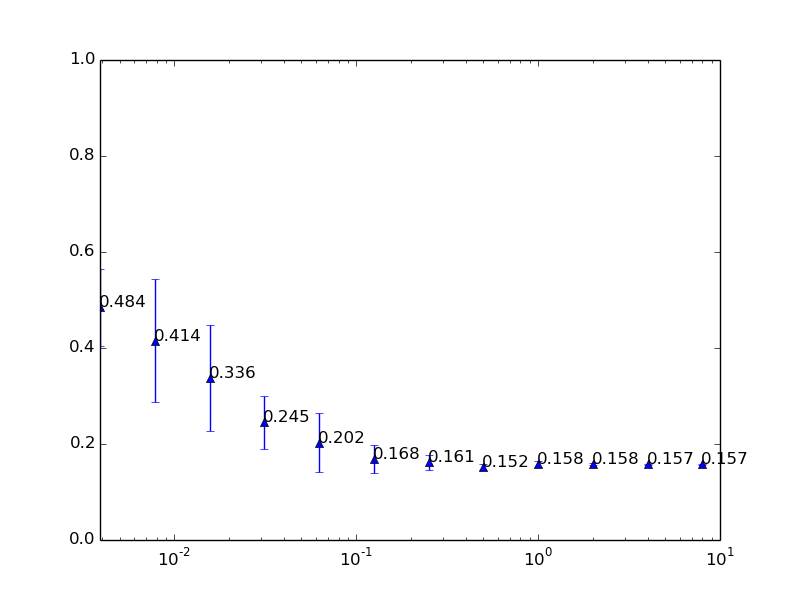
\includegraphics[width=\textwidth]{fig/spambase/eps2e-8-2e8,budg=eps,peers10,groups10,reg2e-2-data368-pubAll-spam-baseline-testset}
	\caption{$\epsilon = [10^{-3}, 10^{3}], \lambda = 2^{-4}$, 50 peers, 1 aggregation}
	\label{fig:epsilon_big_range}
\end{figure}

%testing range of regularization in various settings to validate presence of expected behavior
\begin{figure}[h!]
	\centering
	\begin{minipage}{.49\linewidth}
		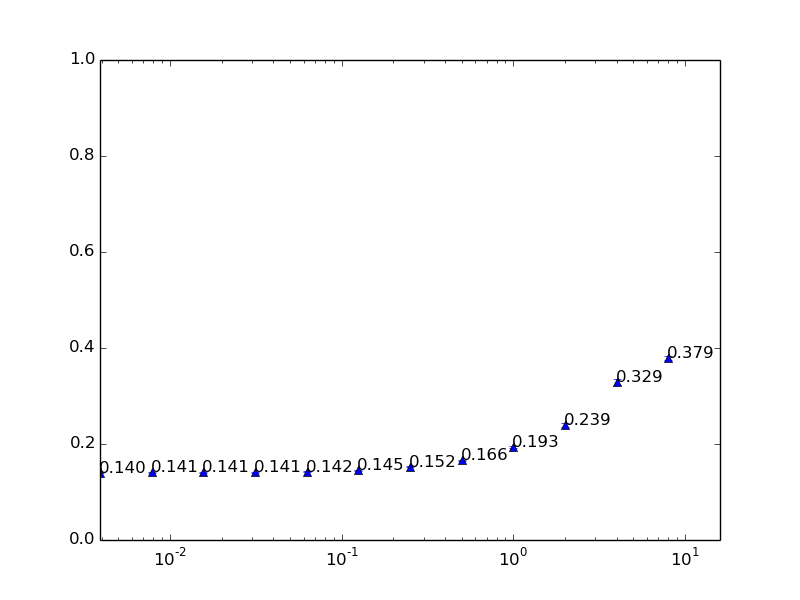
\includegraphics[width=\linewidth]{fig/spambase/eps2e10,budg=eps,peers10,groups10,reg2e-8-2e3-data368-pubAll-spam-baseline-testset}
		\captionof{figure}{$\epsilon = 2^{10}, \lambda = [2^{-8}, 2^{3}]$, 10 peers, 1 aggregation}
		\label{fig:regularization_extremelyhighepsilon}
	\end{minipage}
	\hspace{.001\linewidth}
	\begin{minipage}{.49\linewidth}
		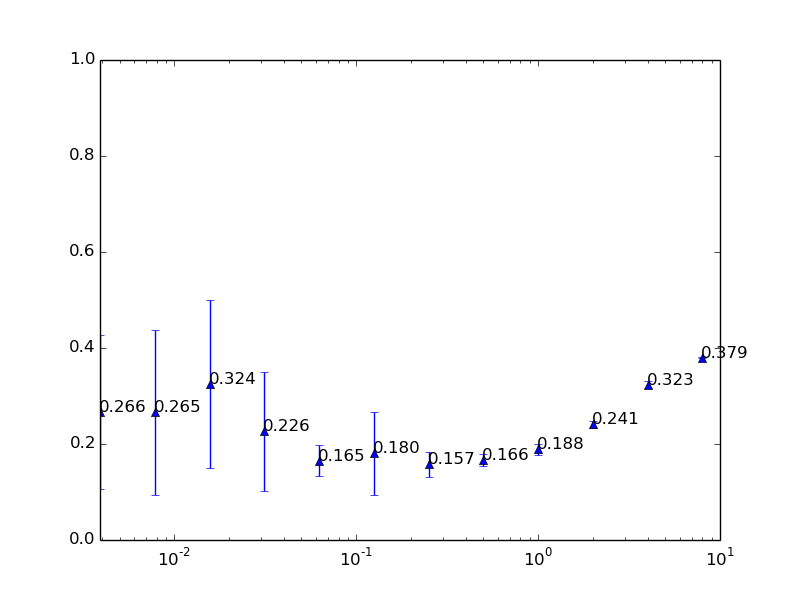
\includegraphics[width=\linewidth]{fig/spambase/eps0.1,budg=eps,peers10,groups10,reg2e-8-2e3-data368-pubAll-spam-baseline-testset}
		\captionof{figure}{$\epsilon = 0.1, \lambda = [2^{-8}, 2^{3}]$, 10 peers, 1 aggregation}
		\label{fig:regularization_normalepsilon}
	\end{minipage}
	\begin{minipage}{.49\linewidth}
		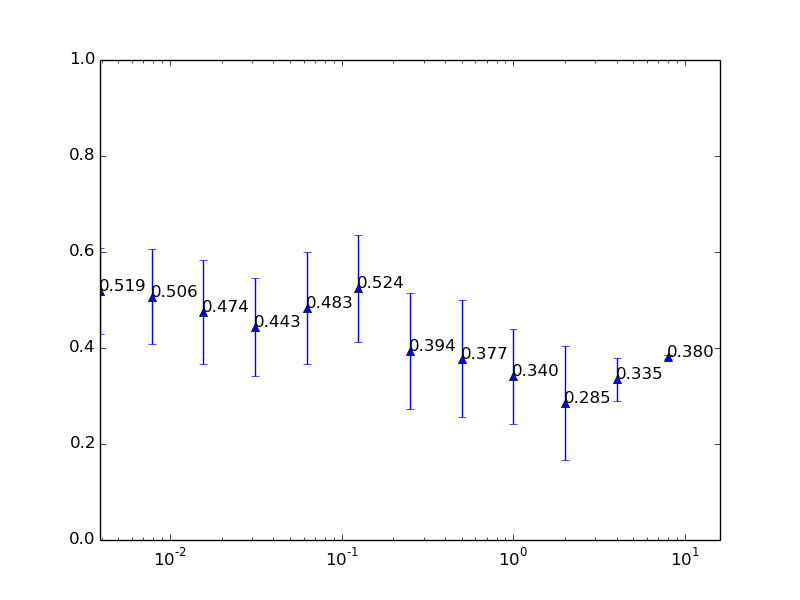
\includegraphics[width=\linewidth]{fig/spambase/eps0.01,budg=eps,peers10,groups10,reg2e-8-2e3-data368-pubAll-spam-baseline-testsetmean}
		\captionof{figure}{$\epsilon = 0.01, \lambda = [2^{-8}, 2^{3}]$, 10 peers, 1 aggregation}
		\label{fig:regularization_lowepsilon}
	\end{minipage}
\end{figure}

%figures showing the effect of data amounts in various combinations of models

\begin{figure}[h!]
	\centering
	\begin{minipage}{.49\linewidth}
		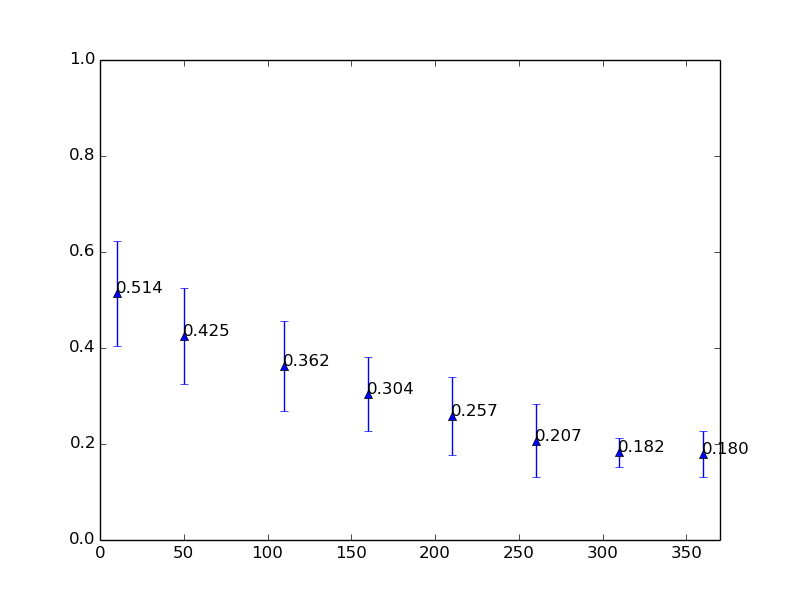
\includegraphics[width=\linewidth]{fig/spambase/eps0.1,budg=eps,peers10,groups10,reg2e-2-pubAll-spam-baseline-data10-360-testset-withoutlocalmodel}
		\captionof{figure}{$\epsilon = 0.1, \lambda = 2^{-2}$, 10 peers, 1 aggregations. Aggregated model only.}
		\label{fig:data_limit_test_withoutlocalmodel}
	\end{minipage}
	\hspace{.001\linewidth}
	\begin{minipage}{.49\linewidth}
		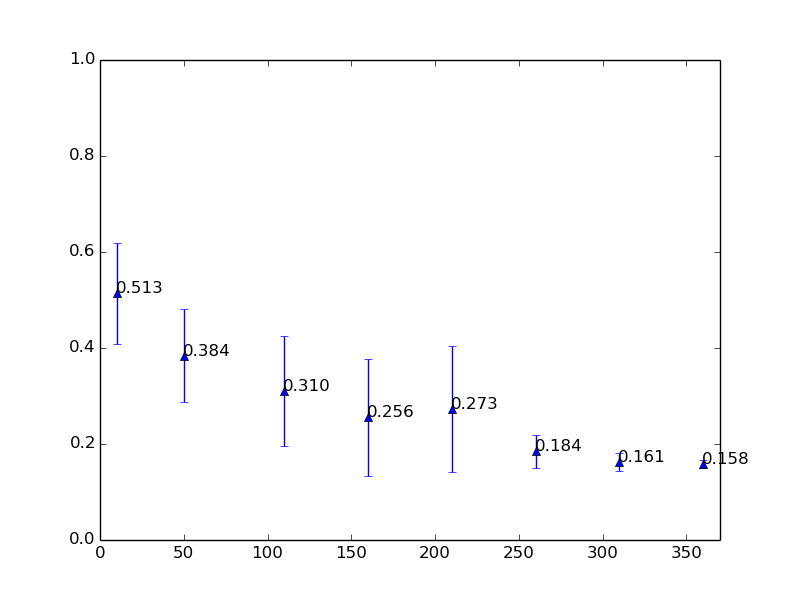
\includegraphics[width=\linewidth]{fig/spambase/eps0.1,budg=eps,peers10,groups10,reg2e-2-pubAll-spam-baseline-data10-360-testset-withlocalmodel}
		\captionof{figure}{$\epsilon = 0.1, \lambda = 2^{-2}$, 10 peers, 1 aggregation. Aggregated and local model.}
		\label{fig:data_limit_test_withlocalmodel}
	\end{minipage}
	\begin{minipage}{.49\linewidth}
		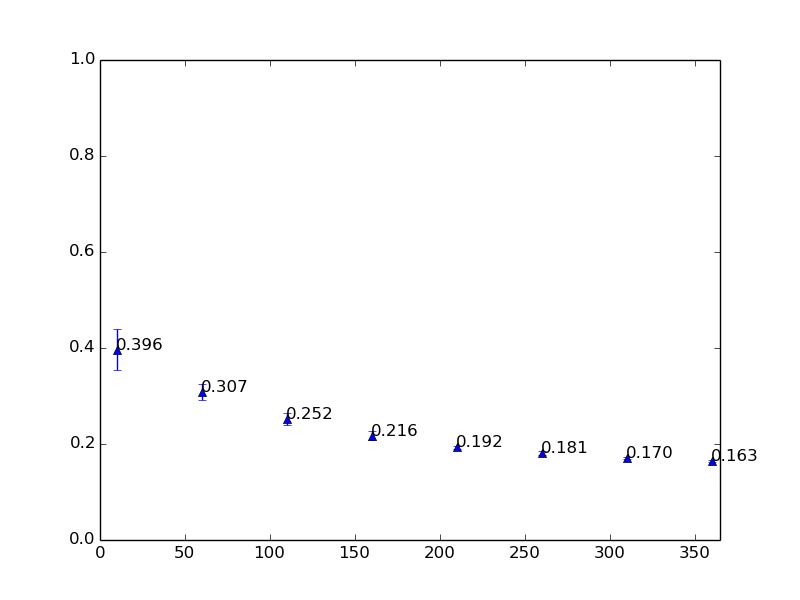
\includegraphics[width=\linewidth]{fig/spambase/eps0.1,budg=eps,peers10,groups10,reg2e-2-pubAll-spam-baseline-data10-360-testset-localmodelonly}
		\captionof{figure}{$\lambda = 2^{-2}$, 10 peers, local model only.}
		\label{fig:data_limit_test_localmodelonly}
	\end{minipage}
\end{figure}

%result of testing constant group size with ever larger number of peers
\todo[inline]{make Effect of peer numbers into a simple table row showing min/max instead}
\begin{figure}[h]
	\centering
	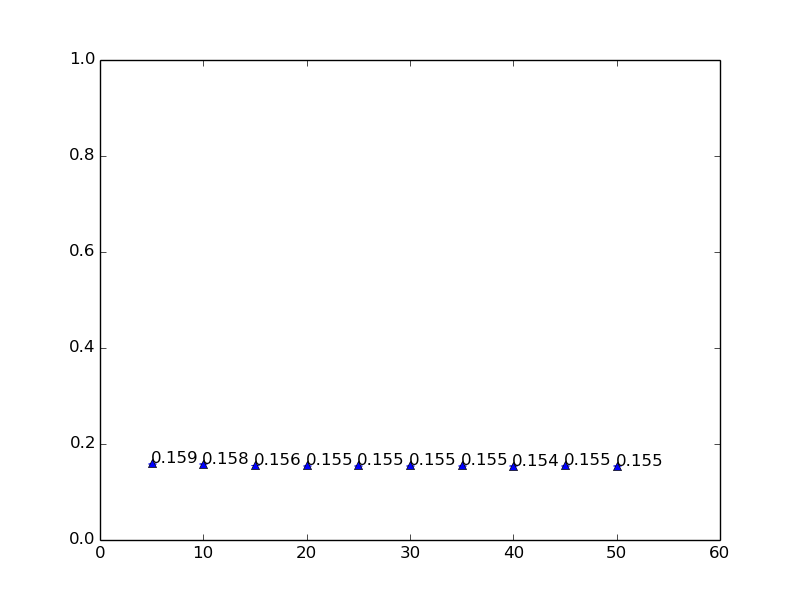
\includegraphics[width=\textwidth]{fig/adult/eps1.0,budg=eps,peers5-55,groups5,reg2e2-data500-pubAll-adult-groupbypeerverification-3-testsetmean}
	\caption{Effect of peer numbers. Group size: 50. Publishing: All. Data: 500}
	\label{fig:peer_range_constant_group}
\end{figure}


%figure showing the presence of variance among peers 
\todo[inline]{replace variance table with numbers from recent, properly CVed runs. ALSO, add std.dev. of std dev. :)}
\begin{table}[h]
	\centering
	\caption{Variance among peers, Adult}
	\label{table:peer_variance_adult}
	\begin{tabular}{|l|l|l|}
		\textbf{Model}                  & \textbf{Mean error} & \textbf{Peer std. dev.} \\
		\hline
		Local, no privacy      & 0,175 & 0.006 \\
		Aggregated, d. privacy & 0,158 & 0.000	 \\
		Ensemble with both & 0.166 & 0.002 \\
	\end{tabular}
\end{table}      

\begin{figure}[h]
	\centering
	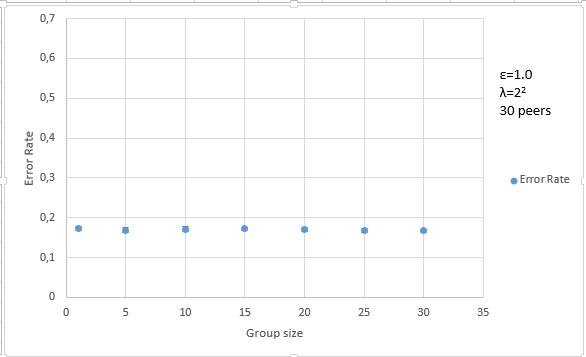
\includegraphics[width=\textwidth]{fig/adult/GroupSizeTest}
	\caption{Effect of Aggregation Group Sizes.}
	\label{fig:results_group_sizes}
\end{figure}

%add - some result comparing difference between party and all publishing


%add - some result showing what happens when group sizes change - maybe combined with the above


\begin{figure}[h]
	\centering
	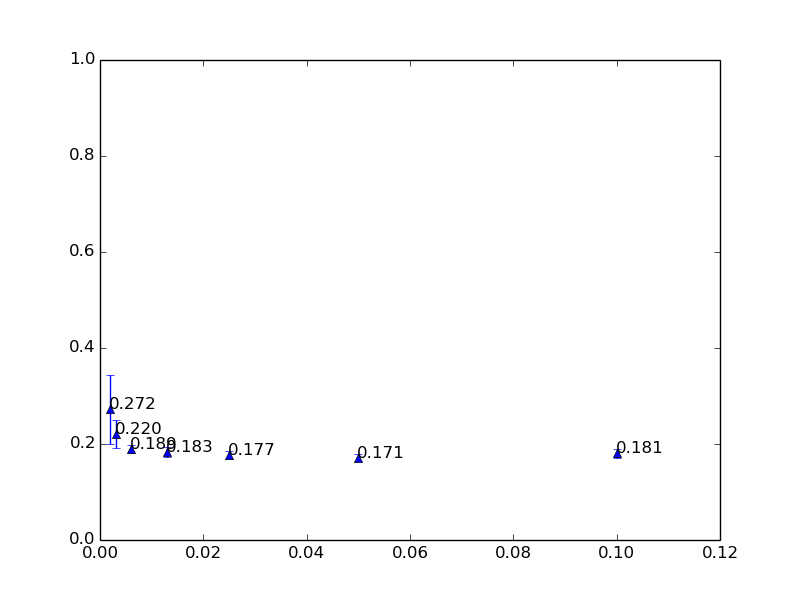
\includegraphics[width=\textwidth]{fig/adult/eps0.1,bud0.1div1-64,peers10,groups2,reg2e2-pubAll-groupsizetest-withoutlocal-data200-adultmean}
	\caption{Effect of Privacy Budgeting.}
	\label{fig:results_privacy_budget}
\end{figure}


%add - some result showing what happens when the amount of privacy budget used is changed - possibly considering all vs party also here


\cleardoublepage